% by pts@fazekas.hu at Fri Aug 28 09:29:30 CEST 2009
%
% !! reorder slides
% !! rename to better reflect not-TeX-only
% !! mark the documents that are by TeX
% !! no colors in the document size chart
% !! add file sizes to the bottom of graph 2
%
% SUXX: pdflatex cannot embed (missing glyph) a Keynote chart with an ff
%       ligature in the caption. Solution: ZERO-WIDH-JOINER unicode char.
\documentclass{beamer}
\usepackage{lmodern}
\usepackage{t1enc}
\usepackage{graphicx}
\usepackage{beamerthemesplit}
\usepackage{ulem}


\definecolor{GoogleBlue}{RGB}{0,102,204}
\definecolor{GoogleRed}{RGB}{255,0,0}
\definecolor{GoogleYellow}{RGB}{255,204,0}
\definecolor{GoogleGreen}{RGB}{0,153,0}
\RequirePackage{xspace}
\newcommand\Google{% The Googley \Google :)
\texorpdfstring{% Color changes do not like to be in bookmarks.
{\color{GoogleBlue}G}%    G
{\color{GoogleRed}o}%     o
{\color{GoogleYellow}o}%  o    :)
{\color{GoogleBlue}g}%    g
{\color{GoogleGreen}l}%   l
{\color{GoogleRed}e}%     e
}{Google}% Colorless text used instead when colors won't work.
\xspace}

\definecolor{c-purple}{rgb}{0.4353,0.2392,0.4745}
\definecolor{c-red}{rgb}{0.7373,0.1765,0.1882}
\definecolor{c-yellow}{rgb}{0.9059,0.6314,0.2392}
\definecolor{c-green}{rgb}{0.3647,0.5882,0.2824}
\definecolor{c-blue}{rgb}{0.1804,0.3412,0.5490}

\title{Optimizing PDF output size of \TeX{} documents}
\subtitle{\ldots{} and PDF files created by other means as well}
\author[P\'eter Szab\'o]{P\'eter Szab\'o\texorpdfstring{\\}{ -- }\textbf{\Google}}
\date{2009-08-31\par\medskip EuroTeX\,2009\\ The Hague, The Netherlands}

%** Create a colorful full square with the specified color.
\def\colorsquare#1{{\color{#1}\vrule width.8em height.8em depth0pt}}

%** Put content to a frame with raggedbottom vertical alignment.
%** This has a hard-coded height for the useful content, depends on the
%** number of sections as well.
%** @example
%**   \frame{
%**      \nocenterframetitle{...}
%**      \nocenter{
%**      ...
%**      }
%**   }
\def\nocenter#1{%
  \hrule height0pt
  \vbox to200pt{\vsize=200pt{\ignorespaces#1}\vfil}%
}

\begin{document}

\frame{\titlepage}

% !!
%\section[Outline]{}
\section{Why and how to optimize?}

\frame{\frametitle{Outline}\tableofcontents}

\subsection{Introduction}

\def\coloremph#1{{\usebeamercolor[fg]{description item}#1}}

\frame{
\frametitle{Why create small PDF files?}
\begin{itemize}
\advance\itemsep1em
\item speed up \coloremph{downloads} (and also reduce download consts)
\item reduce \coloremph{storage} costs (for publishers, book shops,
      libraries and print shops;
      the same PDF is stored at many places)
\item use the capacity of \coloremph{e-book readers} more effectively
\end{itemize}
}

\frame{
\frametitle{Our PDF optimization approach}
Steps:
\begin{enumerate}
\item \coloremph{generate} the PDF as usual, adjusting only a few, crucial settings
\item \coloremph{repeat} if necessary
\item once the final PDF is ready, \coloremph{optimize} it automatically with one
      or more optimizers
\end{enumerate}
Do not:
\begin{itemize}
\item try to improve or fine-tune every PDF creator software
\item lose printable or interactive information while optimizing
\item use a more compact output file format (such as Multiavalent compact PDF)
\item render vector graphics
\end{itemize}
}

\frame{
\frametitle{Proposed workflow}
\begin{enumerate}
\advance\itemsep1em
\item follow the best practices for choosing and configuring the
      \coloremph{\TeX{} driver} (pdf\TeX{}, dvipdfm or
      \sout{dvips} + ps2pdf)
\item if affordable, run commercial optimizer \coloremph{PDF Enhancer} or
      \coloremph{Adobe Acrobat} to optimize content streams
\item run our new optimizer called \coloremph{pdfsizeopt.py}
      mainly to optimize images and Type\,1 fonts\par
      \url{http://code.google.com/p/pdfsizeopt/}
\item use \coloremph{Multivalent} \texttt{tool.pdf.Compress} to do the
      rest of the optimization (done automatically by pdfsizeopt.py)
\end{enumerate}
}

\subsection{Optimization techniques}

\frame{
\frametitle{Local techniques are the most effective}
\begin{itemize}
\advance\itemsep1em
\item remove extra whitespace and comments
\item serialize strings more effectively
\item compress streams with high-effort ZIP (no RLE, LZW and fax anymore)
\item use cross-reference streams (with the \emph{y} predictor)
\item use object streams
\end{itemize}
}

\frame{
\frametitle{Techniques if data types are known}
\begin{itemize}
\advance\itemsep1em
\item get rid of explicitly specified default values
\item remove keys ignored by the PDF specification
\item remove page thumbnails
\item flatten the page structure
\end{itemize}
}

\frame{
\frametitle{Get rid of duplicate and unused data}
\begin{itemize}
\advance\itemsep1em
\item get rid of unused objects (pages, images, anchors etc.)
\item compact the cross-reference tables
\item find duplicate or equivalent objects, and keep only one copy
\item convert some inline images to objects to help deduplication
\item split some large arrays and dictionaries to help deduplication
\item make direct 
\end{itemize}
}

\frame{
\frametitle{Image optimization techniques}
!!
!! get rid of image duplicates based on pixel colors
}

\frame{
\frametitle{Font optimization techniques}
!!
}

\frame{
\frametitle{Advanced content stream techniques}
!!
}

\subsection{For \TeX{} documents}

\frame{
\frametitle{Drivers: dvipdf(x) $<$ pdf\TeX $ll$ dvips }
!!
}

\frame{
\frametitle{Manual setup for small PDF from \TeX{}}
!!
}

\section{Effectiveness measurements}

\subsection{Input PDF files}

\frame{
\frametitle{Input PDF files}
\begin{description}
\item[cff] \emph{CFF reference}; 62 pages; by FrameMaker $+$ Distiller
\item[beamer] first beamer.cls example; 75 slide-steps; by pdf\TeX{}
\item[eu2006] proceedings; 126 pages; by pdf\TeX{} $+$ concat
\item[inkscape] Inkscape manual; 341 pages; by CodeMantra
\item[lme2006] proceedings in Hungarian; 240 pages; by dvips $+$ ps2pdf $+$ concat
\item[pdfref] \emph{PDF\,1.7 reference} 1310 pages; by FrameMaker $+$ Distiller
\item[pgf2] \emph{TikZ manual} 560 pages; by pdf\TeX{}
\item[texbook] \emph{The \TeX{}book} 494 pages; by pdf\TeX{}
\item[tuzv] mini novel in Hungarian; 20 pages; by dvipdfm
\end{description}
}

\frame{
\frametitle{Input PDF sizes}
\nocenter{%
%\vbox to 0pt{}%
%\nointerlineskip
\noindent\hfil
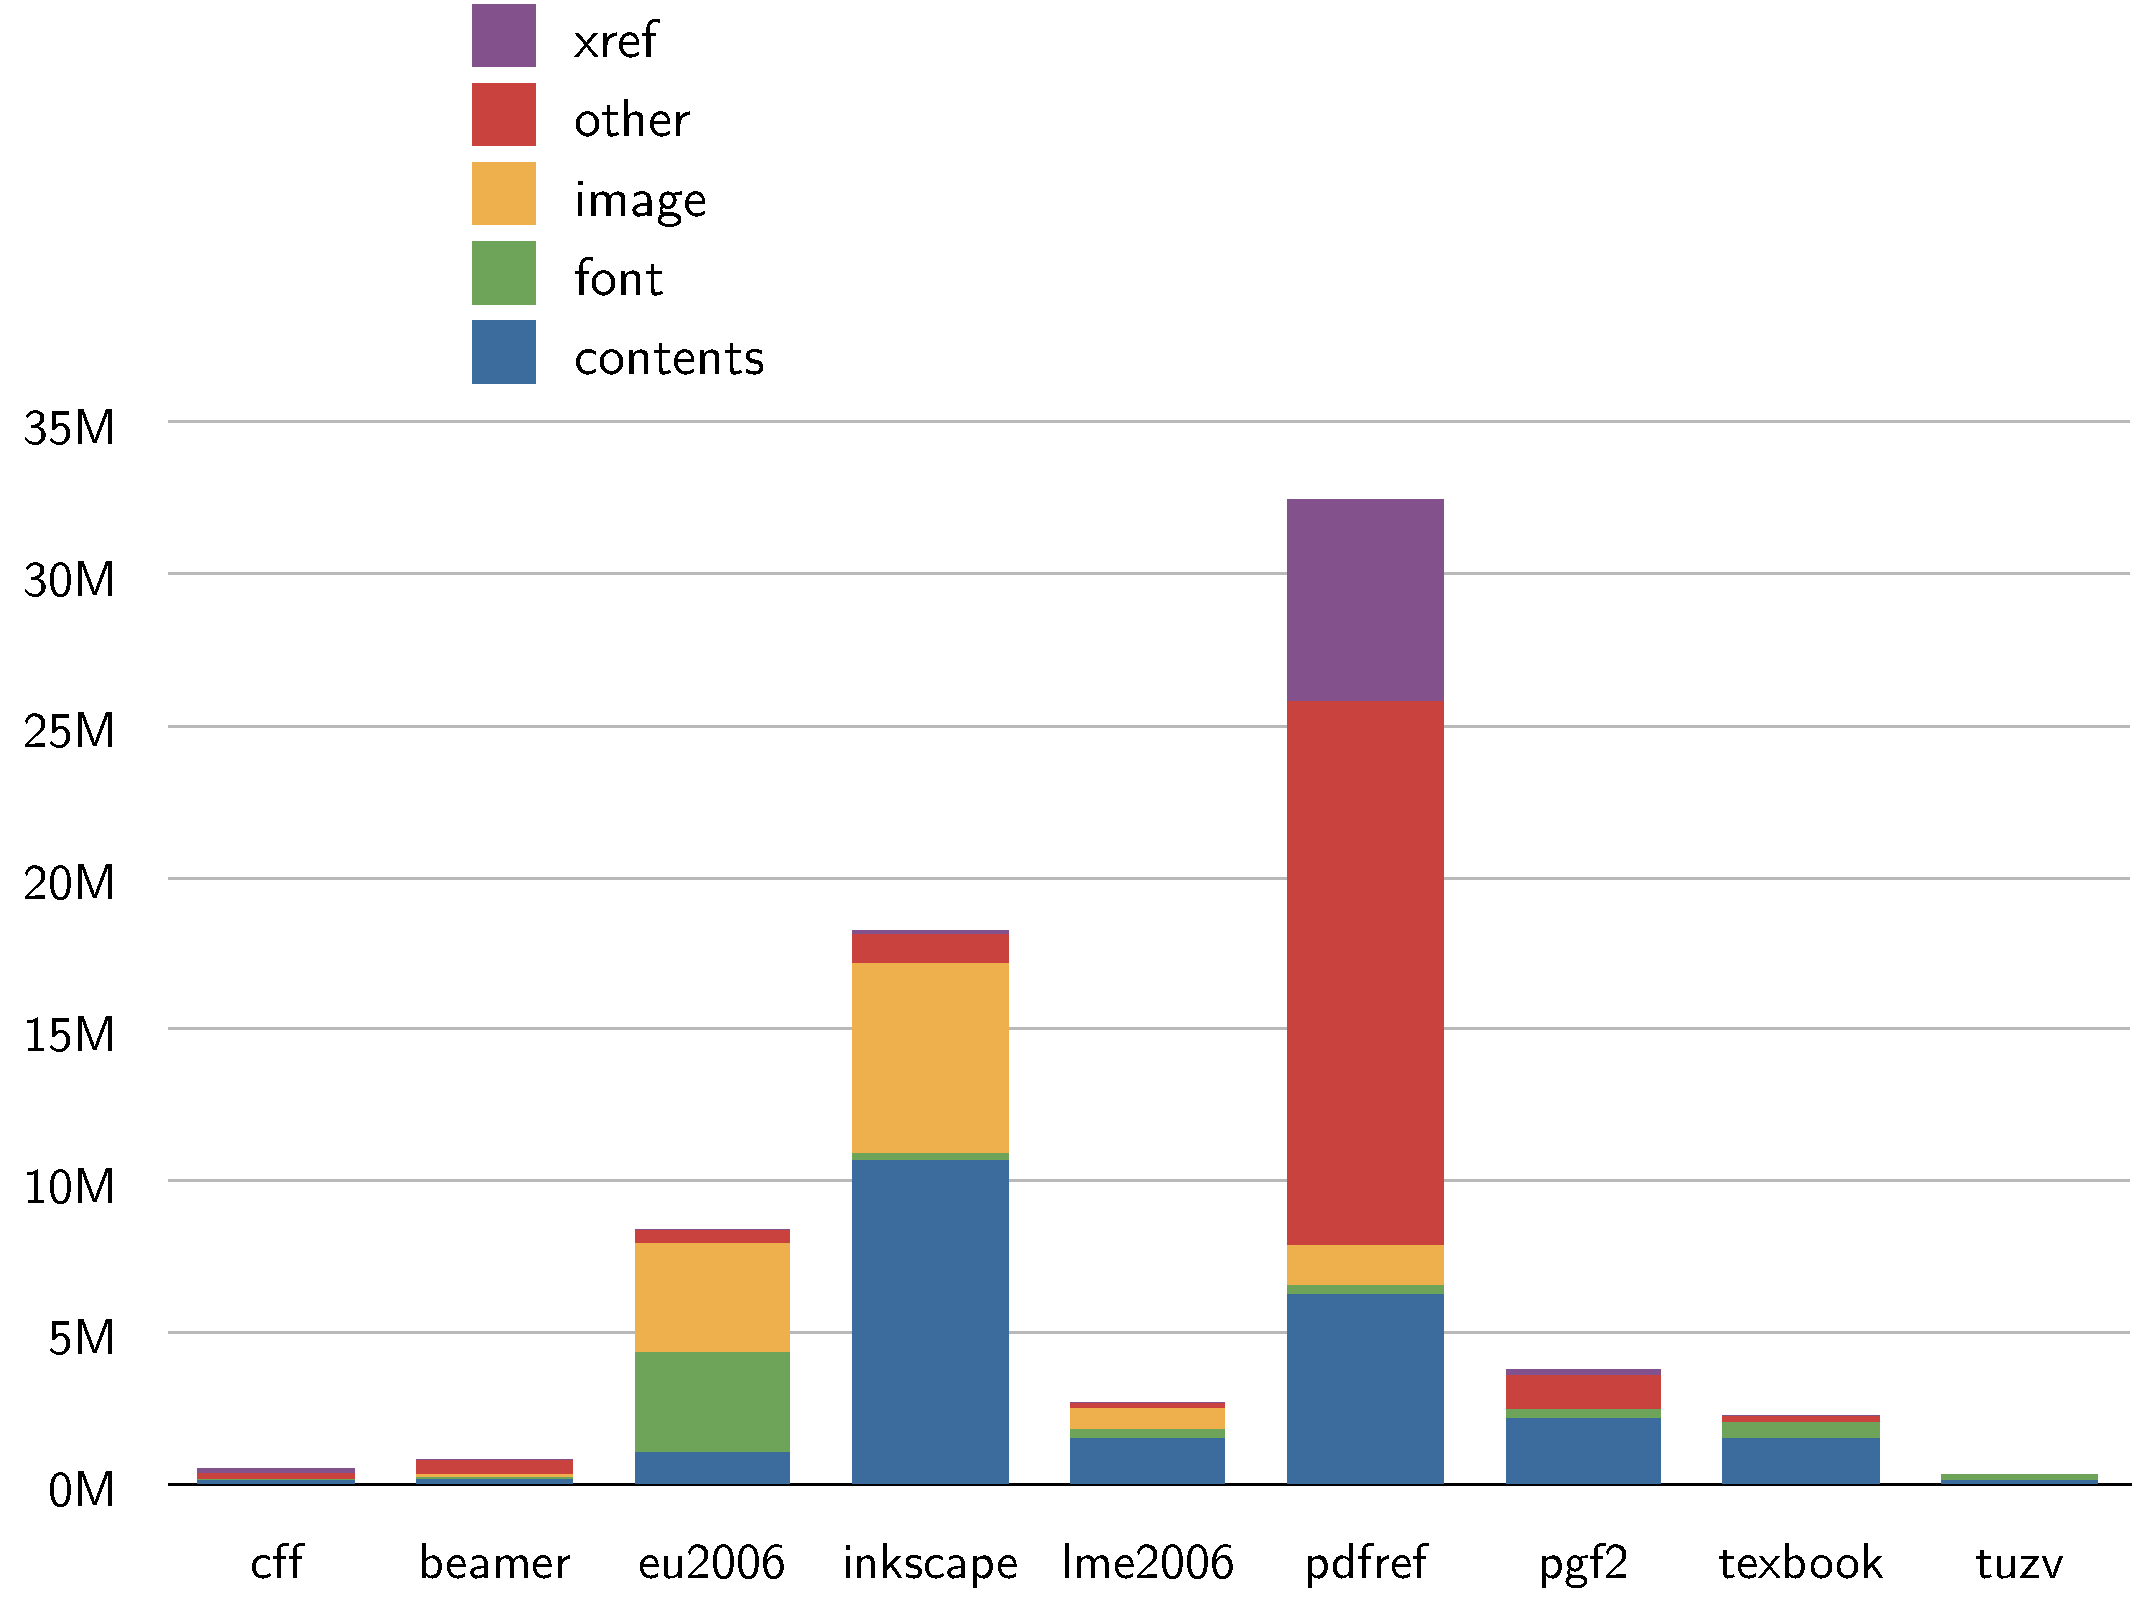
\includegraphics[height=\vsize]{pdfsizeopt_charts.pdf}
}}

\frame{
\frametitle{PDF features measured}
\begin{description}
\item[xref \colorsquare{c-purple}] cross-reference table containing the document offsets
\item[other \colorsquare{c-red}] hyperlinks, anchors, page structure, section structure
(outlines), submittable forms, and other metadata
\item[image \colorsquare{c-yellow}] embedded pixel images (XObject and inline)
\item[font \colorsquare{c-green}] embedded vector font data
\item[contents \colorsquare{c-blue}] vector graphics, text, colors, patterns
etc., including content streams and form XObjects
\end{description}
}

\frame{
\frametitle{Input PDF feature distribution}
\nocenter{%
\noindent\hfil
\includegraphics[height=\vsize,page=2]{pdfsizeopt_charts.pdf}
}}

\subsection{Optimization effectiveness by feature}

%\frame{
%\frametitle{Image optimization effectiveness (byte sizes)}
%\nocenter{%
%\noindent\hfil
%\includegraphics[height=\vsize,page=3]{pdfsizeopt_charts.pdf}
%}}

\frame{
\frametitle{Vector graphics and text optimization effectiveness}
\nocenter{%
\noindent\hfil
\includegraphics[height=\vsize,page=4]{pdfsizeopt_charts.pdf}
}}

\frame{
\frametitle{Embedded font optimization effectiveness}
\nocenter{%
\noindent\hfil
\includegraphics[height=\vsize,page=5]{pdfsizeopt_charts.pdf}
}}

\frame{
\frametitle{Pixel image optimization effectiveness}
\nocenter{%
\noindent\hfil
\includegraphics[height=\vsize,page=6]{pdfsizeopt_charts.pdf}
}}

\frame{
\frametitle{Other data optimization effectiveness}
\nocenter{%
\noindent\hfil
\includegraphics[height=\vsize,page=7]{pdfsizeopt_charts.pdf}
}}

\frame{
\frametitle{Cross-reference optimization effectiveness}
\nocenter{%
\noindent\hfil
\includegraphics[height=\vsize,page=8]{pdfsizeopt_charts.pdf}
}}

\section{Conclusion}

\frame{
\frametitle{Related work}
!!
}

\frame{
\frametitle{Future work}
!!
}

\frame{
\frametitle{Conclusion}
!!
!! most of the size reduction comes from the simplest techniques
}

%\subsection{Overview of the Beamer Class}
%\frame
%{
%  \frametitle{Features of the Beamer Class}
%
%  \begin{itemize}
%  \item<1-> Normal LaTeX class.
%  \item<2-> Easy overlays.
%  \item<3-> No external programs needed.      
%  \end{itemize}
%}

\frame{
\thispagestyle{empty}
%\frametitle{hello}
\noindent\hfill{\fontsize{150}{150}\selectfont?}\hfill\null\par
}

\frame{\thispagestyle{empty}}

\end{document}
